\section{Mutation Analysis}

Attempting to improve a fuzzing effort is one way to find problems
with the effort; if you succeed, you found a weakness.  However, none
of the attempts exposed a serious problem.  Adding more fuzzers would
be \emph{good}, but was not obviously \emph{essential}.  Ensemble
fuzzing was not feasible, and swarm testing was, for practical
purposes, already performed by alternative means.  An alternative is
to directly look for holes in testing.  The Bitcoin Core fuzzing team
clearly was measuring and inspecting code coverage (see \url{https://marcofalke.github.io/btc_cov/}), so little value
would be added by inspecting traditional coverage alone.  Mutation
testing/analysis~\cite{MutationSurvey,budd1979mutation,demillo1978hints}, however, subsumes code coverage and adds extremely
valuable information on \emph{oracle power} in addition to mere
coverage~\cite{Discontents}.  This is perhaps especially valuable in fuzzing, where ``you
only see crashes'' is a persistent concern.  In previous work, we had
used mutation testing to improve the random testing of the Linux
kernel's RCU module, and in the process discovered some subtle kernel bugs~\cite{mutKernel,groce2018verified}.

\begin{sloppypar}
We used the universal mutator
\noindent(\url{https://github.com/agroce/universalmutator})~\cite{regexpMut}, a
mutation tool already used widely in the blockchain and smart contract world, to
mutate the Bitcoin and other popular cryptocurrencies core transaction
verification code. We focused on transaction verification code, as it is generally well-covered by
tests, and obviously an extremely critical functionality for the blockchain.
\end{sloppypar}

\subsection{Mutation Testing Bitcoin}

\begin{sloppypar}

To perform mutation analysis on Bitcoin, we generated mutations for code in the
{\tt tx\_verify.cpp} file. We then evaluated the ability of fuzzing and testing
to detect such mutants. Figure~\ref{kills} summarizes our mutation
analysis of the file.

\begin{figure}
\vspace{2mm}
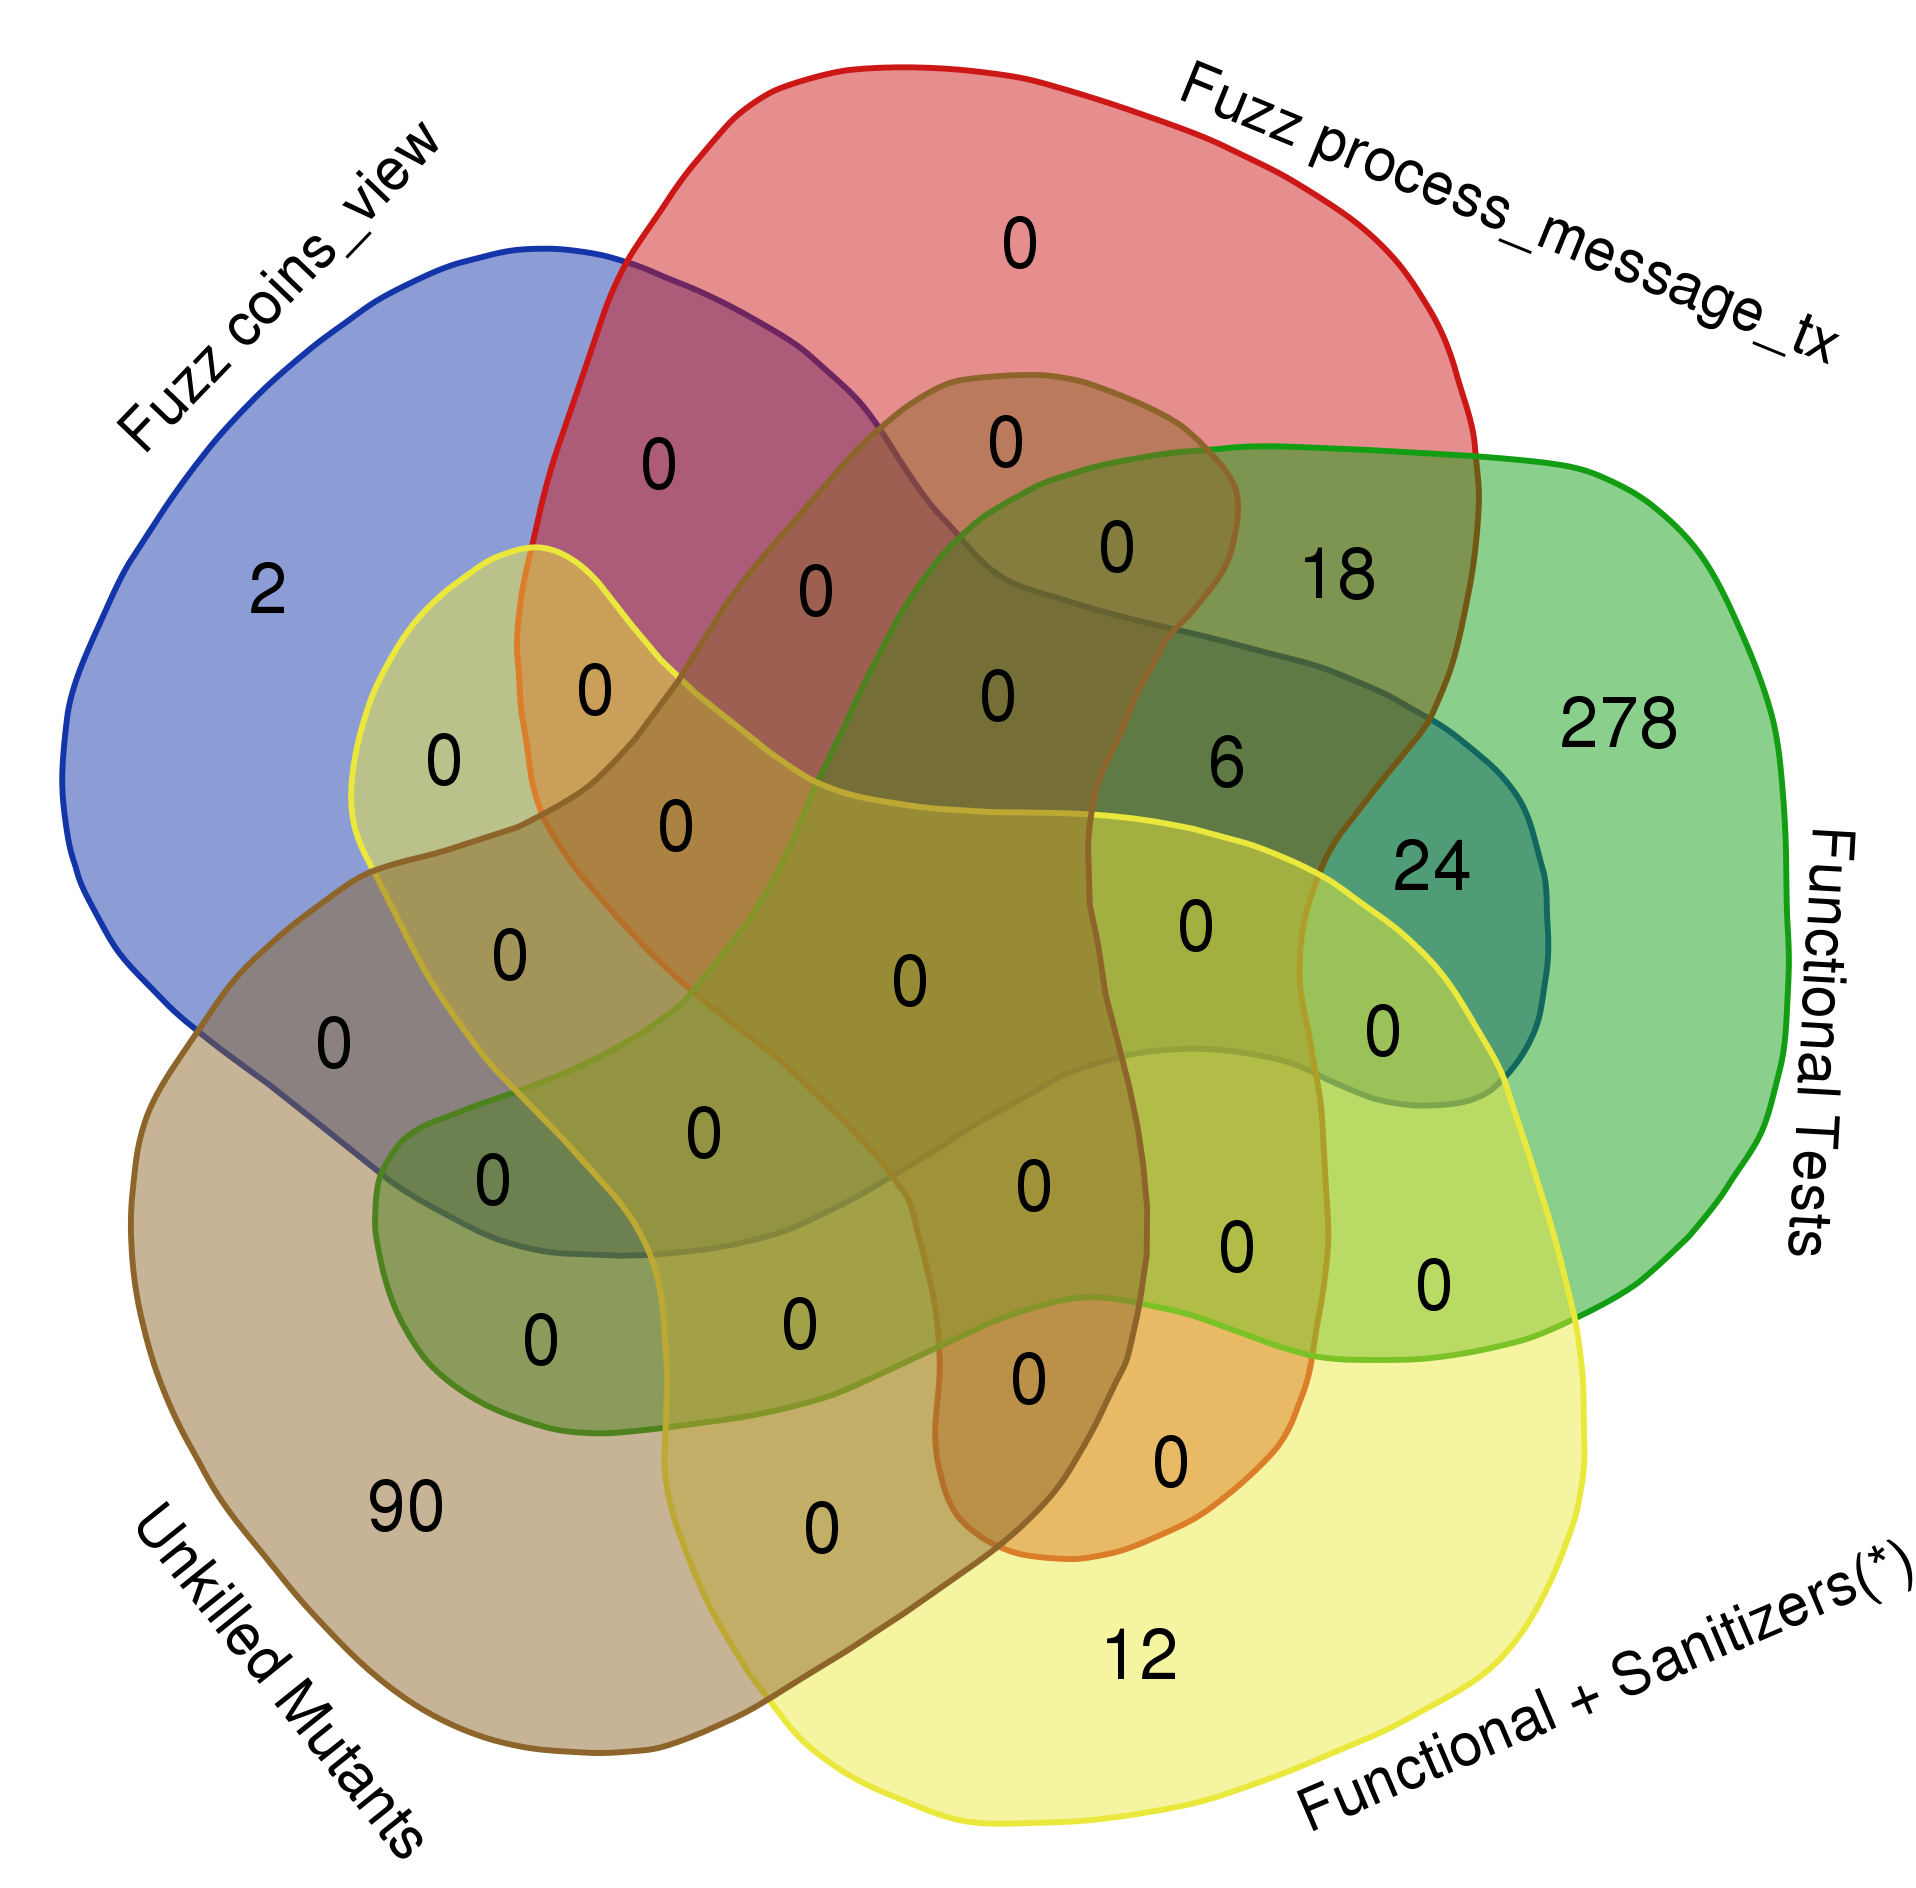
\includegraphics[width=0.9\columnwidth]{kill_pre_valgrind.png}
\caption{A comparison of mutation kills for {\tt tx\_verify.cpp} when subjected to different testing and fuzzing parameters.}
\label{kills}
\end{figure}

\begin{figure*}
\raggedright
  
{\bf Original mutated code (and immediate context):}
  
\begin{code}
    if (coin.IsCoinBase() \&\& nSpendHeight - coin.nHeight < COINBASE\_MATURITY) \{
            return state.Invalid(TxValidationResult::TX\_PREMATURE\_SPEND, "bad-txns-premature-spend-of-coinbase",
                strprintf("tried to spend coinbase at depth \%d", nSpendHeight - coin.nHeight));
\end{code}

{\bf Mutant \#379} changes the {\tt strprintf} to:

\begin{code}
strprintf("tried to spend coinbase at depth \%d", nSpendHeight / coin.nHeight));
\end{code}
      
{\bf Mutant \#380} changes the {\tt strprintf} to:      

\begin{code}
strprintf("tried to spend coinbase at depth \%d", nSpendHeight \% coin.nHeight));
\end{code}
\caption{Mutants detected \emph{only} by fuzzing.}
\label{mkills}
\end{figure*}

The universal mutator generated 430 compiling mutants of the file in
less than three hours\footnote{Building all test and fuzz targets for each
candidate mutant takes some time, and parallelizing the task would
require multiple sandboxed copies of the code. Constructing a more
focused build command than {\tt make -j5}, that avoids building most tests, might speed this up substantially}.
Two functions with interesting tests overlapped with our fuzzing targets in {\tt
  tx\_verify.cpp} code: {\tt process\_message\_tx} and {\tt coins\_view}.
Additional functions {\tt process\_message} and {\tt process\_messages} were
also fuzz tested and of potential interest, but the relevant corpus entries were
duplicated in {\tt process\_message\_tx} (we verified these provided no
additional mutant kills). We ran fuzzing for five minutes using
libFuzzer exploration based on the full (and large) QA asset corpus for each
harness, with all sanitizers enabled. The {\tt process\_message\_tx} target was
able to detect 24 mutants, and the {\tt coins\_view} harness was able to detect
32 mutants, for a total of 50 mutants. In other words, slightly short of 12\%
over all the generated mutants. This is not a bad result: fuzzing inherently has
trouble detecting subtle, non-crash-inducing, bugs in code, because writing a
strong specification of correct behavior that covers all the bizarre and
pointless inputs produced in fuzzing is often impractical, or would require a
specification nearly as complex as the code itself. This is one reason
\emph{differential} fuzzing is promising: a reference implementation is such a
specification. Bitcoin Core's cryptographic elements are, in fact,
differentially fuzzed
\url{https://github.com/bitcoin/bitcoin/pull/22704#issuecomment-898989809}.
\end{sloppypar}


A major purpose of fuzzing is, then, to address limits in more
traditional functional testing, where known inputs are paired with
expected behavior.  While functional or unit testing is very powerful,
the kinds of bugs found in vulnerabilities often involve the kind of
inputs that don't appear in ``normal'' unit/functional tests, as shown
by the success of fuzzing and security audits~\cite{FC20}.  The real
question, then, is how many mutants that survive Bitcoin Core's
extensive functional tests survive fuzzing.

The answer is: not too many.  The functional tests without sanitizers
enabled catch an additional 278 mutants.  Turning on sanitizers (which
is very expensive --- we \emph{only} ran it for mutants surviving all other
tests, as indicated by the zero overlap and the asterisk in Figure~\ref{kills}) catches an additional 12 mutants.  Only 90 of the
430 compiling mutants survive all tests, for an overall mutation score
of 79.07\%.

Fuzzing adds two unique mutant kills beyond those produced by
the functional testing.  Figure~\ref{mkills} shows the (very similar
code) for these two mutants.  Only fuzzing generates inputs that cause
{\tt coin.nHeight} to be zero.  Fuzzing doesn't increase code coverage
here, but does increase interesting \emph{data value} coverage.  Use
of the libFuzzer {\tt -use\_value\_profile=1} flag is likely
instrumental in achieving such good value coverage.  Adding that flag was
one of the first suggestions in the 80-hour effort, but it turned out
this was already standard practice in the Bitcoin Core fuzz configuration.


Manual inspection of the surviving mutants showed that at
least 29 of these were clearly semantically equivalent to the
un-mutated code.  For instance, many mutants removed or weakened an
assertion; clearly this cannot ever be detected, since it can only
transform failing tests into passing tests.  The full, detailed list
of surviving mutants, prioritized by an FPF ranking~\cite{10.1145/2491956.2462173,Gonzalez85}, is
available here:
\url{https://github.com/agroce/bitcorpus/blob/master/mutation/prioritized_full_inspect.txt}.
Discussion with the Bitcoin Core team is ongoing as we write
(\url{https://github.com/bitcoin/bitcoin/issues/22690}), but thus far
none of the surviving mutants seem to expose serious testing
problems.  After manual pruning, the mutation score is 85.8\%, and
some of the remaining 61 mutants are likely also equivalent.  The
limitations of the fuzzing oracle are clear: fuzzing covers 98\% of
statements and 72.6\% of branches as we write, but can kill fewer than
12\% of mutants.  The much greater killing power of the functional
tests obviously does not lie in the marginal 0.7 percentage points and 0.5
percentage points of statement and branch coverage obtained; it lies
in the ability to reject incorrect executions that do not crash or set
off a sanitizer alarm.

This raises the question:  why fuzz?  The coverage for high quality
(if imperfect) functional tests such as those for Bitcoin Core will
often be considerably
higher, and the oracle will almost always be \emph{much} more powerful.  The answer lies in the
fact that, even in the presence of such high quality tests, fuzzing
uncovers subtle bugs that functional tests designed by humans will
almost never detect,
e.g. \url{https://github.com/bitcoin/bitcoin/issues/22450}\footnote{Comments
  on this bug, such as ``Another win for fuzzing, oh wow.'' and
  ``Fuzzer rulez!'' show that the Bitcoin Core team has little doubt
  about the power of fuzzing.}.  Fuzzing is \emph{not} a replacement
for functional/unit tests; and functional/unit tests are not a
replacement for fuzzing.  In our mutation analysis, consider the two
mutants detected by {\tt coins\_view} fuzzing alone.  In the
traditional, score-based, view of mutation analysis, the {\tt
  coins\_view} fuzz harness would be seen as performing badly.  But it
detects 2 (hypothetical) bugs not detectable by other means; in the
real world, if one such bug is exploitable, detecting it may ``pay
for'' all the fuzzing effort, and there will seldom be just one such
bug (see
\url{https://github.com/bitcoin/bitcoin/issues?q=is\%3Aissue+fuzz+is\%3Aclosed+label\%3ABug}
for an approximate list of fuzzer-detected, fixed bugs in Bitcoin
Core).  If the ``good guys'' don't fuzz well, you can be sure the bad
guys will, for software protecting billions of dollars of assets.

\subsection{Other Cryptocurrency Projects}

% for solana, these are app.codecov.io/gh/solana-labs/solana @a6a4cfd numbers. grcov
% doesn't include tests, but reports coverage % as a total over lines including
% tests, so it's also not accurate. we'll just over approximate rather than
% underapproximate and acknowledge that in the text
\begin{table*}[ht!]
\vspace{2mm}
\centering
\begin{tabular}{llrccc}
\toprule
\bf \mr{2}{Project}             & \bf \mr{2}{File path}                         & \bf \mr{2}{LOC}  & \mc{1}{c}{\bf Mutation} & \mc{1}{c}{\bf File}     & \mc{1}{c}{\bf Project}   \\
\bf                             & \bf                                           & \bf              & \mc{1}{c}{\bf score}    & \mc{1}{c}{\bf coverage} & \mc{1}{c}{\bf coverage}  \\
\midrule
bitcoin                         & src/consensus/tx\_verify.cpp                  & 210              & 78.6\%                  & 98.7\%                  & 84.2\%                   \\
\cmidrule{2-6}
\mr{3}{go-ethereum}             & core/block\_validator.go                      & 129              & 70.1\%                  & 81.0\%                  &  \mr{3}{58.8\%}          \\
                                & signer/fourbyte/validation.go                 & 127              & 49.5\%                  & 60.0\%                  &                          \\
                                & signer/core/signed\_data.go                   & 1,044            & 25.3\%                  & 69.3\%                  &                          \\
\cmidrule{2-6}
\mr{3}{solana}                  & perf/src/sigverify.rs                         & 1,246            & ????\%                  & 74.48\%                 & \mr{3}{82.2\%}           \\
%                               & core/src/sigverify\_stage.rs                  & 296              & ????\%                  & 88.46\%                 & \mr{3}{82.2\%}           \\  this seems to just call perf/src/sigverify
                                & core/src/validator.rs                         & 2,016            & -                       & 73.29\%                 &                          \\
                                & core/src/tvu.rs                               &  494             & -                       & 63.12\%                 &                          \\
\cmidrule{2-6}
dogecoin                        & src/bitcoin-tx.cpp                            & 847              & 58.7\%                  & -                       & 70.1\%                   \\
\cmidrule{2-6}
avalanchego                     & vms/platformvm/add\_subnet\_validator\_tx.go  & 308              & 57.3\%                  & 81.0\%                  & 63.6\%                   \\
\cmidrule{2-6}
  stellar                       & src/historywork/VerifyTxResultsWork.cpp       & 192              & 85.1\%                  & -                       & -                        \\
\cmidrule{2-6}
go-algorand                     & ledger/eval.go                                & 1,551            & 99.8\%                  & 86.0\%                  & 52.2\%                   \\
\cmidrule{2-6}
cosmos-sdk                      & x/auth/ante/sigverify.go                      & 510              & 73.1\%                  & -                       &  -                       \\
\bottomrule
\end{tabular}
\caption{Code Coverage and Mutation Scores Across Popular Cryptocurrencies. \underline{Mutation score} represents the proportion of mutants that were killed divided by the total number of mutants (higher is better).
\underline{File coverage} and \underline{Project coverage} report statement level coverage for the file and entire project, respectively. \underline{LOC} represents the lines of code of the chosen file. Absent entries indicated by \texttt{-} means we could not
obtain coverage data, or otherwise curbed additional experiments.
\rvt{rvt asks: what do we want to say about inception date here, or in the text? i presume there's something interesting to say here since we're including the data...}}
\label{tab:comparison}
\end{table*}


\begin{table*}[ht!]
\vspace{2mm}
\centering
\begin{tabular}{llcc}
\toprule
\bf Mutation Operator                          & \bf Project and File                  & \bf Old Code                              & \bf New Code              \\
\midrule
Comment out source code line                   & bitcoin - tx\_verify.cpp              & \textcd if (!MoneyRange(coin.out.nValue) || !MoneyRange(nValueIn)) {
!             return state.Invalid(TxValidationResult::TX\_CONSENSUS, "bad-txns-inputvalues-outofrange");
          }                                    &                           \\
bitcoin                                        &                                       &                                           &                           \\
bitcoin                                        &                                       &                                           &                           \\
bitcoin                                        &                                       &                                           &                           \\
\bottomrule
\end{tabular}
\caption{Sample of Mutation Rules and Examples for Various Cryptocurrencies that were not killed.}
\label{tab:rules}
\end{table*}

\begin{figure}
\vspace{2mm}
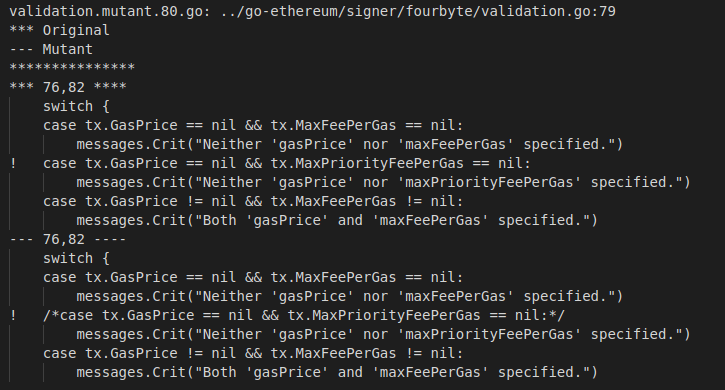
\includegraphics[width=0.9\columnwidth]{mutation-example.png}
\caption{Mutation Example for Ethereum Transaction Validation}
\label{fig:mutation}
\end{figure}

\begin{figure}
\vspace{2mm}
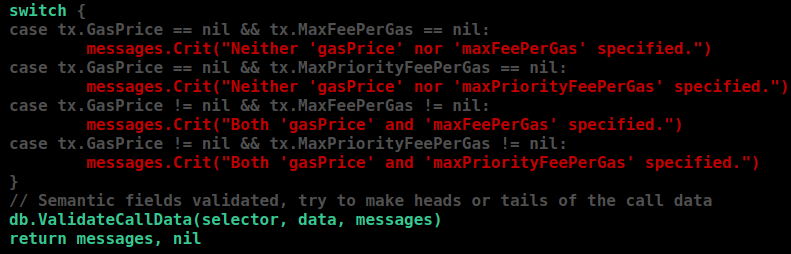
\includegraphics[width=0.9\columnwidth]{coverage-example.png}
\caption{Coverage Example for Ethereum Transaction Validation}
\label{fig:coverage}
\end{figure}

Our Bitcoin work prompted mutation analysis for other popular cryptocurrencies.
We generated mutants using the universal mutator for code in Ethereum, Solana,
Dogecoin, Avalanche, Stellar, Algorand, and Cosmos, a selection from the top 30
cryptocurrencies\footnote{By market capitalization according to
\url{https://coinmarketcap.com}.} Our selection is influenced by the
availability of code coverage, and indicative of the further opportunities for
mutation testing in Bitcoin and popular altcoins, rather than a
comprehensive survey. Because it requires significant effort to set up or
otherwise understand the extent of fuzz testing in this heterogeneous selection
of projects, our mutation analysis here only considers pure mutation testing
against the project test suite (no fuzzing).

For the same reasons above, we targeted transaction validation logic and
identified candidate files by searching for keywords like \texttt{transaction},
\texttt{verify}, \texttt{sign}, and \texttt{validate}. We manually inspected
functions and test coverage for these functions (where applicable) to identify
which files would be interesting targets to generate mutants for. Ultimately we
settled on one to three files per project that are representative of some
interesting and tested functionality (a choice that we readily acknowledge is by
no means comprehensive or suggestive of a project's quality and testing as a
whole).

\subsubsection*{Experimental Setup}
\rvt{rvt says: a TODO here that answers:
- what is the range of number of mutants we generated across all projects (min and max)
- how long did mutant generation take?
- how many mutation operators (or ``rules'') were used?
- where they the same or different for each project?
}
We ran the universal mutator on the candidate files above, using both the universal rules and
language specific rules. There were 92 universal rules (transformations that can apply to
any language) and between 0 and 20 language specific rules, depending on the source language
of the project. One can view these rules 
at \url{https://github.com/agroce/universalmutator/tree/master/universalmutator/static}.

Using these rules, we generated mutant candidates. The number of generated mutants varied depending
on the source language and length of the candidate file, ranging from 492 (go-ethereum's block\_validator.go) to 
8567 (go-ethereum's signed\_data.go) mutants. Following the generation of mutants, the universal mutator
executed these candidate mutants against each project's test suite, reporting mutation score. The runtime
of this also varied based on test execution time of project and number of candidate mutants, ranging from
42 minutes (go-ethereum's validation.go) to 32 hours (dogecoin's bitcoin-tx.cpp).

\subsubsection*{Experimental Results.}

\rvt{rvt says: a TODO to address in this subsection, or elsewhere above as examples of mutation testing: a handful of example mutants and/or mutation operators (either those that were unkilled by the Bitcoin runs, or the ones we did in our altcoin experiments) in the form of a readable table or something like that. i think would be really interesting to the reader. e.g., ``what kinds of mutation operators did we decide on? which kinds of mutants survived?''. even if it's standard stuff, it's probably not something the reader wants to guess about, and really is a ``oh that's interesting'' kind of thing to look at. we have the figures but it's difficult to read and these are really trying to make a different point (See discussion) so a table with mutation operators/rules or examples would be awesome}

Table~\ref{tab:comparison} summarizes our results, which lists the
\textbf{Mutation score}, \textbf{File coverage}, and \textbf{Project coverage}
over the selected file. \textbf{Mutation score} represents the proportion of
mutants that were killed by the project's test suite divided by the total number
of mutants (higher is better). File and project metrics represent statement
coverage. statement level. In principle, we expect that higher file coverage
(i.e., more tested code) to correlate with a higher mutation score.\rvt{don't
  know if this needs a cite but that seems intuitive, sort of?}

Out of our selection, Bitcoin's mutation score ranks high. Our experience
working with Bitcoin Core developers show that they are proactive about code
quality and testing, which is likely to influence (whether directly or
indirectly) mutation scores.\rvt{question for Alex: are we comfortable saying
  something along these lines? just an attempt to reword what the previous
  sentence here tries to convey. otherwise, let's cut it} At the same time, code
around transaction verification and validation may naturally vary depending on
context, code organization, and language as reflected by the differences in
lines of code in our selection (and unknown function dependencies or testing in
the rest of the codebase). Thus, the extent of our mutation testing per file
ultimately serve as individual datapoints that are difficult to compare
horizontally across projects. \rvt{rvt says: changed things because basically
  like, cool, bitcoin is high, but like, we're mutating a 210 line file and it
  has lots of calls to lots of other code and the mutation score could be lower
  or higher if we decided to mutation test something somewhere else along the
  callchain that a tx\_verify operation operates on. we really really can't say
  with confidence or even speculate (IMO) that this mutation score is super meaningful if we're tempted
to compare it to other projects. Not even Doge fork because it's not the same file? If it were the same file I might feel differently.
% Previous text:
%
% Interestingly, bitcoin seems to have among the highest coverage and mutation
% score out of any of the popular cryptocurrencies, with even forks of bitcoin,
% such as dogecoin having both lower project coverage and mutation score.
}


% Secondly, other than go-ethereum, none of the cryptocurrencies besides bitcoin
% employed any kind of fuzzing, with bitcoin employing continuous fuzzing through
% OSS fuzz to catch bugs.
%
% rvt says: the part about others not doing fuzzing isn't true, at least not based on searching for `fuzz` in other projects:
% stellar: https://sourcegraph.com/search?q=repo:%5Egithub%5C.com/stellar/stellar-core%24+fuzz&patternType=literal
% algorand: https://sourcegraph.com/search?q=repo:%5Egithub%5C.com/algorand/go-algorand%24+fuzz&patternType=literal
% cosmos: https://sourcegraph.com/search?q=repo:%5Egithub%5C.com/cosmos/cosmos-sdk%24+fuzz&patternType=literal
%
% don't think we can confidently state the part about continuous fuzzing either, and i don't think we have much to gain from this anyway. at best "maybe fuzzing influences/correlates with mutation testing but like probably that's a very weak connection as per the other text in this paper"

% RVT commenting this out because wee're saying this up front now
%
% Furthermore, there does seem to be a correlation between coverage and mutation score, with files with high coverage typically killing the majority of the generated mutants.

Investigating files with lower coverage (e.g., those in Ethereum), we noticed
that many of the generated mutants removed lines related to error checking
(e.g., in switch case statements) that were apparently not covered by tests (cf.
Figures \ref{fig:mutation} and \ref{fig:coverage}).

% RVT says: there may be a chance that the switch case statements are not covered for other reasons (disabled tests, bad coverage tool). Likely these are untested, but I think it's fine to just state our observations.
%
% The lack of coverage of these exceptional cases across ethereum and many other low coverage files we examined, % was something that surprised us, as we expected these files to have high coverage
% and test both happy and exceptional paths.

\subsubsection*{Considerations for further study.}

Unit tests and corresponding coverage reports, while useful in our context of
mutation testing, contribute only to one aspect of code quality and ignores
other kinds of testing. Incorporating integration and differential tests with
coverage would deliver deeper insights of under-tested code and overall code quality.

In a similar vein, we limited our mutation testing to a handful of files based
on a convenience sample. A deeper mutation analysis with a higher allocation of
resources (perhaps justifying resources comparable to fuzz testing) poses interesting
possibilities that may allow more direct comparison and contrast among projects.

\iffalse
% RVT comments this out because I think we can sidestep the whole thing about "did we pick other targets well and how does it compare to bitcoin" because we really can't compare it anyway, so let's just say "we picked other targets and here's what we see".
One potential limitation of our analysis is the selection of files relating to transaction and block validation. While our heuristics and manual inspection did lead us to files that fulfilled these
properties, they were not comprehensive in finding all relevant files.
Particularly in cryptocurrencies, such as ethereum, there is no one file that
handles all transaction or block validation (a file analagous to {\tt
  tx\_verify.cpp} in bitcoin), but rather this logic is spread over dozens of
different files. As a result, we are not able to make any definitive claims
about the quality of these test suites, but rather observations regarding
mutation score and how good bitcoin's overall mutation score is.

Finally, the bulk of our time was spent investigating bitcoin, making us most
familiar with its codebase. There is a possibility that we may have missed
certain tests in other cryptocurrencies, as even in bitcoin the functional tests
were not well-documented and difficult to find as a third party.

Furthermore, another limitation was that we spent more time was spent investigating bitcoin than any other cryptocurrency, meaning that there is a chance that we missed
some test that were not documented or easy to find in other cryptocurrencies.
\fi
